Plastic scintillators are easy to machine to any desired shape. The chosen shape for TRITIUM detector is the fiber, specifically, commercial fibers BCF-12 from Saint-Gobain Crystals Inc \cite{DataSheetBCF12Fiber}. This type of fiber was chosen as the result of a comparative study \cite{TFGAlberto} among some of the best-known commercial manufacturers. The BCF-12 fibers consist of scintillating polystyrene with the posibility of surounding it by a cladding of polymethylmethacrylate (PMMA) (smaller refractive index than core in order to archieve a critical angle) or a multicladding (second cladding) with even smaller refractive index.

When a particle deposits all or part of its kinetic energy, some photons are produced in the fiber core as a result of the scintillating process. The number of photons produced depend on the scintillation efficiency and its value is around $2.4\%$ for the fibers used (BCF-12), which means that a scintillation yield of about $8000$ photons will be produced per $\MeV$ for a mip. For instance, for tritium electrons, these fibers release a maximum of around 148 photons (when a tritium electron has the maximum energy, $18.6~\keV$), or less as electrons of these energies are not mips. The emission spectrum of the fibers employed in this work, is shown in Figure \ref{fig:EmissionSpectrumFibers}.

\begin{figure}[htbp]
\centering
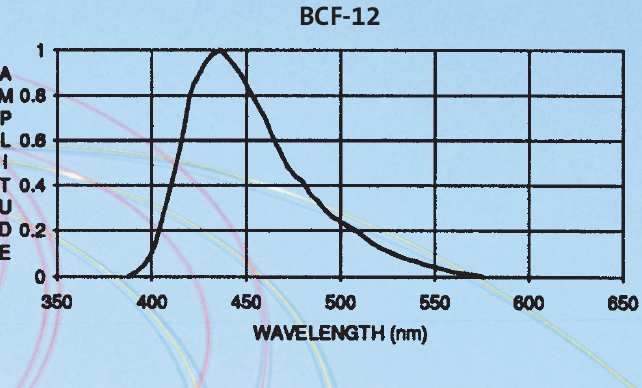
\includegraphics[scale=0.5]{3DesignPrinciples/32Tritium_detector/EmisionBCF12.png}
\caption{Emission spectrum of BCF-12 fibers of Saint-Gobain\label{fig:EmissionSpectrumFibers}~\cite{DataSheetBCF12Fiber}.}
\end{figure}

The scintillation light is guided to the sensitive part of the photosensor. A single photon produces a signal with some probability, called the quantum efficiency. Fibers (and scintillators in general) use the optical property of Snell's law \cite{Snell} to guide their photons to the desired part (ends of the fibers). The guiding mechanism is based on the interface created between the core and the surrounding material. When a photon hits this interface, it is refracted (and therefore lost) following the Snell equation, \ref{eq:Snell} \cite{Snell}. 

\begin{equation}
n_0~sen(\theta_0) = n_1~sen(\theta_1) \longrightarrow \theta_c = asen\left(\frac{n_1}{n_0} \right)
\label{eq:Snell}
\end{equation}
If the surrounding material has a lower refractive index than the core of the fiber, there exist a critical angle, $\theta_c$, beyond which photons will be totally reflected and therefore kept within the fiber as illustrated in Figure \ref{fig:Fiber_physic}.

The trapping efficiency or photon collection efficiency is defined as the efficiency of the scintillator to guide photons. For BCF-12 fibers with optical clad this efficiency is between $3.44\%$ and $7\%$ per meter of fiber (depending on where the event is detected and is minimum near the fiber axis  and maximum near the core-clad interface). For uncladded fibers BCF-12 surrounded by water, the trapping efficiency is larger than for cladded fibers. Therefore, from the maximum of $148$ photons initially created by a tritium decay electron with the maximum energy, only 41 photons (for maximum trapping efficiency) are guided along the $25~\cm$ fiber length of the TRITIUM detector. Thus, the output signal is very weak and is in the range of the spectrum where electronic noise is already significant. As described in the following chapters, a great effort was made to minimize electronic noise by different techniques. In Figure \ref{fig:Fiber_physic} the light collection in a fiber is illustrated.

\begin{figure}[htbp]
\centering
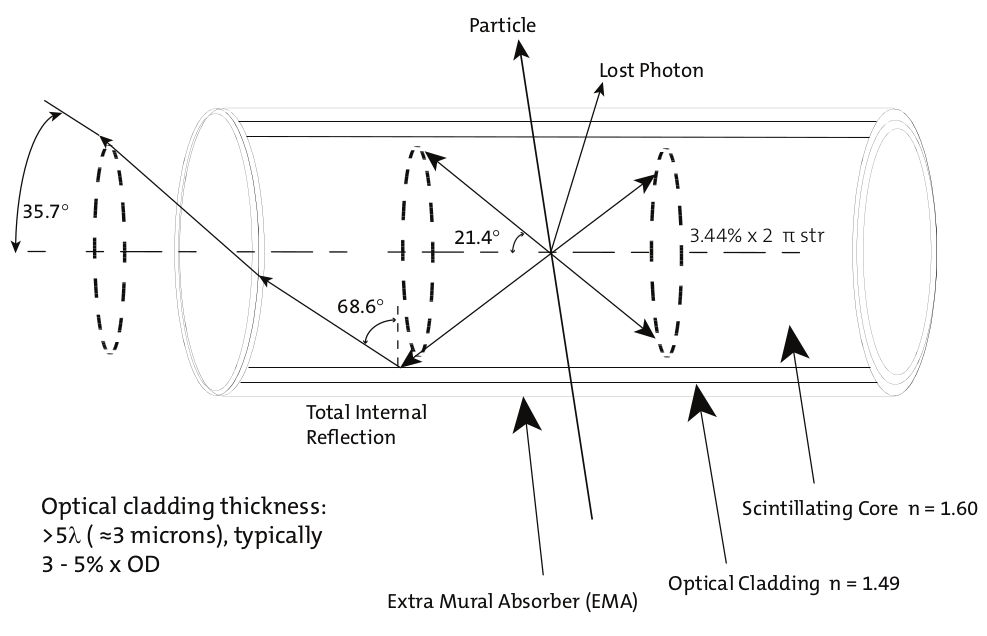
\includegraphics[scale=0.5]{3DesignPrinciples/32Tritium_detector/Fiber_data_sheet.png}
\caption{Photon collection in a single clad fiber\label{fig:Fiber_physic}~\cite{DataSheetBCF12Fiber}.}
\end{figure}

The cladding material is useful for protecting the core surface from dirt or aggressive external agents that may reduce the light collection but at the cost of increasing the critical angle with its corresponding loss of light. Three different cases are shown in Table \ref{tab:CriticalAngles}, where the cladding effect is ilustrated.

\begin{table}[htbp]
%%\centering
\begin{center}
\begin{tabular}{|c|c|c|}
\hline
Material & Refractive index & critical angle ($\degree$) \\
\hline \hline \hline
Air & 1 & $42.98$ \\ \hline
Water & 1.33 & $62.47$ \\ \hline
Cladding of PMMA & 1.49 & $76.26$ \\ \hline
\end{tabular}
\caption{Critical angles associated to different interfaces created with polystyrene, $n_0=1.6$, and other materials.}
\label{tab:CriticalAngles}
\end{center}
\end{table}

In the practice, it is difficult to achieve a perfect air-core or water-core interface, and this affects light collection. As commercial claddings are thicker ($30~\micro \meter$) than the mean free path of tritium decay electrons in water (around $5~\micro\meter$) cladded fibers is not an option for the TRITIUM detector. Hence, special attention is needed for achieving a water-core interface good enough. To achieve this goal a special protocol was developed in the ICMOL laboratory for preparing fibers for tritium detection, detailed and tested in section \ref{subsec:CleaningProcess}. The most important parameters of scintillating fibers of TRITIUM are given in Table \ref{tab:ParametersFibersBCF12}.

\begin{table}[h]
%%\centering
\begin{center}
\begin{tabular}{|c|c|c|}
%\hline
%Material & Refractive index \\
\hline \hline 
Core material & Polystyrene \\ \hline
Core refractive index & 1.60 \\ \hline
Density ($\gram/\cm^3$) & 1.05 \\ \hline
Cladding material & Acrylic (PMMA) \\ \hline
Cladding refractive index & 1.49 \\ \hline
Cladding thickness ($\mu\meter$) & 30 \\ \hline
Numerical aperture & 0.58 \\ \hline
Trapping efficiency & 3.44\% minimum \\ \hline
No. of H atoms per cc (core) & $4.82 \cdot{} 10^{22}$ \\ \hline
No. of C atoms per cc (core) & $4.85 \cdot{} 10^{22}$ \\ \hline
No. of electrons per cc (core) & $3.4 \cdot{} 10^{23}$ \\ \hline
Radiation lenght (cm) & 42 \\ \hline
Emission peak (nm) & 435 (Blue) \\ \hline
Decay Time, (ns) & 3.2 \\ \hline
1/e Length (m) & 2.7 \\ \hline
Scintillator yield (\#$\gamma$/MeV) & $\sim 8000$ \\ \hline
Operating Temperature & $-20\degree C$ to $50\degree C$ \\ \hline
\end{tabular}
\caption{Properties of BCF-12 fibers from Saint-Gobain Inc. \cite{DataSheetBCF12Fiber}.}
\label{tab:ParametersFibersBCF12}
\end{center}
\end{table}

%Bunch -> manojo de fibras

%bundle -> haz de fibras